\documentclass[11pt,twoside,letterpaper]{article}
\newcommand{\reporttitle}{Lab 2: Closed loop control of mobile robots}
\newcommand{\reportauthorOne}{Adams, Hunter}
\newcommand{\cidOne}{20997503}
\newcommand{\reportauthorTwo}{Chen, Joe}
\newcommand{\cidTwo}{20998545}
\newcommand{\reportauthorThree}{Wielowieyski, Jacob}
\newcommand{\cidThree}{21004619}
\newcommand{\robotNumber}{9 and 16}
\newcommand{\stationNumber}{151}
\date{\today}
%%%%%%%%%%%%%%%%%%%%%%%%%%%%%%%%%%%%%%%%%
% University Assignment Title Page 
% LaTeX Template
% Version 1.0 (27/12/12)
%
% This template has been downloaded from:
% http://www.LaTeXTemplates.com
%
% Original author:
% WikiBooks (http://en.wikibooks.org/wiki/LaTeX/Title_Creation)
%
% License:
% CC BY-NC-SA 3.0 (http://creativecommons.org/licenses/by-nc-sa/3.0/)
% 
% Instructions for using this template:
% This title page is capable of being compiled as is. This is not useful for 
% including it in another document. To do this, you have two options: 
%
% 1) Copy/paste everything between \begin{document} and \end{document} 
% starting at \begin{titlepage} and paste this into another LaTeX file where you 
% want your title page.
% OR
% 2) Remove everything outside the \begin{titlepage} and \end{titlepage} and 
% move this file to the same directory as the LaTeX file you wish to add it to. 
% Then add \input{./title_page_1.tex} to your LaTeX file where you want your
% title page.
%
%----------------------------------------------------------------------------------------
%	PACKAGES AND OTHER DOCUMENT CONFIGURATIONS
%----------------------------------------------------------------------------------------
\usepackage{ifxetex}
\usepackage{textpos}
\usepackage{natbib}
\usepackage{kpfonts}
\usepackage[letterpaper,hmargin=2.8cm,vmargin=2.0cm,includeheadfoot]{geometry}
\usepackage{ifxetex}
\usepackage{stackengine}
\usepackage{tabularx,longtable,multirow,subfigure,caption}%hangcaption
\usepackage{fncylab} %formatting of labels
\usepackage{fancyhdr}
\usepackage{color}
\usepackage[tight,ugly]{units}
\usepackage{url}
\usepackage{float}
\usepackage[english]{babel}
\usepackage{amsmath}
\usepackage{graphicx}
\usepackage[colorinlistoftodos]{todonotes}
\usepackage{dsfont}
\usepackage{epstopdf} % automatically replace .eps with .pdf in graphics
\usepackage{natbib}
\usepackage{backref}
\usepackage{array}
\usepackage{latexsym}
\usepackage{etoolbox}

\usepackage{enumerate} % for numbering with [a)] format 



\ifxetex
\usepackage{fontspec}
\setmainfont[Scale=.8]{OpenDyslexic-Regular}
\else
\usepackage[pdftex,pagebackref,hypertexnames=false,colorlinks]{hyperref} % provide links in pdf
\hypersetup{pdftitle={},
  pdfsubject={}, 
  pdfauthor={\reportauthorOne},
  pdfkeywords={}, 
  pdfstartview=FitH,
  pdfpagemode={UseOutlines},% None, FullScreen, UseOutlines
  bookmarksnumbered=true, bookmarksopen=true, colorlinks,
    citecolor=black,%
    filecolor=black,%
    linkcolor=black,%
    urlcolor=black}
\usepackage[all]{hypcap}
\fi

\usepackage{tcolorbox}

% various theorems
\usepackage{ntheorem}
\theoremstyle{break}
\newtheorem{lemma}{Lemma}
\newtheorem{theorem}{Theorem}
\newtheorem{remark}{Remark}
\newtheorem{definition}{Definition}
\newtheorem{proof}{Proof}

% example-environment
\newenvironment{example}[1][]
{ 
\vspace{4mm}
\noindent\makebox[\linewidth]{\rule{\hsize}{1.5pt}}
\textbf{Example #1}\\
}
{ 
\noindent\newline\makebox[\linewidth]{\rule{\hsize}{1.0pt}}
}



%\renewcommand{\rmdefault}{pplx} % Palatino
% \renewcommand{\rmdefault}{put} % Utopia

\ifxetex
\else
\renewcommand*{\rmdefault}{bch} % Charter
\renewcommand*{\ttdefault}{cmtt} % Computer Modern Typewriter
%\renewcommand*{\rmdefault}{phv} % Helvetica
%\renewcommand*{\rmdefault}{iwona} % Avant Garde
\fi

\setlength{\parindent}{0em}  % indentation of paragraph

\setlength{\headheight}{14.5pt}
\pagestyle{fancy}
\fancyfoot[ER,OL]{\thepage}%Page no. in the left on
                                %odd pages and on right on even pages
\fancyfoot[OC,EC]{\sffamily }
\renewcommand{\headrulewidth}{0.1pt}
\renewcommand{\footrulewidth}{0.1pt}
\captionsetup{margin=10pt,font=small,labelfont=bf}


%--- chapter heading

\def\@makechapterhead#1{%
  \vspace*{10\p@}%
  {\parindent \z@ \raggedright %\sffamily
        %{\Large \MakeUppercase{\@chapapp} \space \thechapter}
        %\\
        %\hrulefill
        %\par\nobreak
        %\vskip 10\p@
    \interlinepenalty\@M
    \Huge \bfseries 
    \thechapter \space\space #1\par\nobreak
    \vskip 30\p@
  }}

%---chapter heading for \chapter*  
\def\@makeschapterhead#1{%
  \vspace*{10\p@}%
  {\parindent \z@ \raggedright
    \sffamily
    \interlinepenalty\@M
    \Huge \bfseries  
    #1\par\nobreak
    \vskip 30\p@
  }}
  



% %%%%%%%%%%%%% boxit
\def\Beginboxit
   {\par
    \vbox\bgroup
	   \hrule
	   \hbox\bgroup
		  \vrule \kern1.2pt %
		  \vbox\bgroup\kern1.2pt
   }

\def\Endboxit{%
			      \kern1.2pt
		       \egroup
		  \kern1.2pt\vrule
		\egroup
	   \hrule
	 \egroup
   }	

\newenvironment{boxit}{\Beginboxit}{\Endboxit}
\newenvironment{boxit*}{\Beginboxit\hbox to\hsize{}}{\Endboxit}



\allowdisplaybreaks

\makeatletter
\newcounter{elimination@steps}
\newcolumntype{R}[1]{>{\raggedleft\arraybackslash$}p{#1}<{$}}
\def\elimination@num@rights{}
\def\elimination@num@variables{}
\def\elimination@col@width{}
\newenvironment{elimination}[4][0]
{
    \setcounter{elimination@steps}{0}
    \def\elimination@num@rights{#1}
    \def\elimination@num@variables{#2}
    \def\elimination@col@width{#3}
    \renewcommand{\arraystretch}{#4}
    \start@align\@ne\st@rredtrue\m@ne
}
{
    \endalign
    \ignorespacesafterend
}
\newcommand{\eliminationstep}[2]
{
    \ifnum\value{elimination@steps}>0\leadsto\quad\fi
    \left[
        \ifnum\elimination@num@rights>0
            \begin{array}
            {@{}*{\elimination@num@variables}{R{\elimination@col@width}}
            |@{}*{\elimination@num@rights}{R{\elimination@col@width}}}
        \else
            \begin{array}
            {@{}*{\elimination@num@variables}{R{\elimination@col@width}}}
        \fi
            #1
        \end{array}
    \right]
    & 
    \begin{array}{l}
        #2
    \end{array}
    &%                                    moved second & here
    \addtocounter{elimination@steps}{1}
}
\makeatother

%% Fast macro for column vectors
\makeatletter  
\def\colvec#1{\expandafter\colvec@i#1,,,,,,,,,\@nil}
\def\colvec@i#1,#2,#3,#4,#5,#6,#7,#8,#9\@nil{% 
  \ifx$#2$ \begin{bmatrix}#1\end{bmatrix} \else
    \ifx$#3$ \begin{bmatrix}#1\\#2\end{bmatrix} \else
      \ifx$#4$ \begin{bmatrix}#1\\#2\\#3\end{bmatrix}\else
        \ifx$#5$ \begin{bmatrix}#1\\#2\\#3\\#4\end{bmatrix}\else
          \ifx$#6$ \begin{bmatrix}#1\\#2\\#3\\#4\\#5\end{bmatrix}\else
            \ifx$#7$ \begin{bmatrix}#1\\#2\\#3\\#4\\#5\\#6\end{bmatrix}\else
              \ifx$#8$ \begin{bmatrix}#1\\#2\\#3\\#4\\#5\\#6\\#7\end{bmatrix}\else
                 \PackageError{Column Vector}{The vector you tried to write is too big, use bmatrix instead}{Try using the bmatrix environment}
              \fi
            \fi
          \fi
        \fi
      \fi
    \fi
  \fi 
}  
\makeatother

\robustify{\colvec}

%%% Local Variables: 
%%% mode: latex
%%% TeX-master: "notes"
%%% End: 

% quick way of adding a figure
\newcommand{\fig}[3]{
 \begin{center}
 \scalebox{#3}{\includegraphics[#2]{#1}}
 \end{center}
}

%\newcommand*{\point}[1]{\vec{\mkern0mu#1}}
\newcommand{\ci}[0]{\perp\!\!\!\!\!\perp} % conditional independence
\newcommand{\point}[1]{{#1}} % points 
\renewcommand{\vec}[1]{{\boldsymbol{{#1}}}} % vector
\newcommand{\mat}[1]{{\boldsymbol{{#1}}}} % matrix
\newcommand{\R}[0]{\mathds{R}} % real numbers
\newcommand{\Z}[0]{\mathds{Z}} % integers
\newcommand{\N}[0]{\mathds{N}} % natural numbers
\newcommand{\nat}[0]{\mathds{N}} % natural numbers
\newcommand{\Q}[0]{\mathds{Q}} % rational numbers
\ifxetex
\newcommand{\C}[0]{\mathds{C}} % complex numbers
\else
\newcommand{\C}[0]{\mathds{C}} % complex numbers
\fi
\newcommand{\tr}[0]{\text{tr}} % trace
\renewcommand{\d}[0]{\mathrm{d}} % total derivative
\newcommand{\inv}{^{-1}} % inverse
\newcommand{\id}{\mathrm{id}} % identity mapping
\renewcommand{\dim}{\mathrm{dim}} % dimension
\newcommand{\rank}[0]{\mathrm{rk}} % rank
\newcommand{\determ}[1]{\mathrm{det}(#1)} % determinant
\newcommand{\scp}[2]{\langle #1 , #2 \rangle}
\newcommand{\kernel}[0]{\mathrm{ker}} % kernel/nullspace
\newcommand{\img}[0]{\mathrm{Im}} % image
\newcommand{\idx}[1]{{(#1)}}
\DeclareMathOperator*{\diag}{diag}
\newcommand{\E}{\mathds{E}} % expectation
\newcommand{\var}{\mathds{V}} % variance
\newcommand{\gauss}[2]{\mathcal{N}\big(#1,\,#2\big)} % gaussian distribution N(.,.)
\newcommand{\gaussx}[3]{\mathcal{N}\big(#1\,|\,#2,\,#3\big)} % gaussian distribution N(.|.,.)
\newcommand{\gaussBig}[2]{\mathcal{N}\left(#1,\,#2\right)} % see above, but with brackets that adjust to the height of the arguments
\newcommand{\gaussxBig}[3]{\mathcal{N}\left(#1\,|\,#2,\,#3\right)} % see above, but with brackets that adjust to the height of the arguments
\DeclareMathOperator{\cov}{Cov} % covariance (matrix) 
\ifxetex
\renewcommand{\T}[0]{^\top} % transpose
\else
\newcommand{\T}[0]{^\top}
\fi
% matrix determinant
\newcommand{\matdet}[1]{
\left|
\begin{matrix}
#1
\end{matrix}
\right|
}



%%% various color definitions
\definecolor{darkgreen}{rgb}{0,0.6,0}

\newcommand{\blue}[1]{{\color{blue}#1}}
\newcommand{\red}[1]{{\color{red}#1}}
\newcommand{\green}[1]{{\color{darkgreen}#1}}
\newcommand{\orange}[1]{{\color{orange}#1}}
\newcommand{\magenta}[1]{{\color{magenta}#1}}
\newcommand{\cyan}[1]{{\color{cyan}#1}}


% redefine emph
\renewcommand{\emph}[1]{\blue{\bf{#1}}}

% place a colored box around a character
\gdef\colchar#1#2{%
  \tikz[baseline]{%
  \node[anchor=base,inner sep=2pt,outer sep=0pt,fill = #2!20] {#1};
    }%
}%

\usepackage{booktabs}
\geometry{left=0.7in,right=0.7in,top=0.55in,bottom=0.55in,headheight=14.5pt,headsep=10pt,footskip=20pt}
\setlength{\headwidth}{\textwidth}
\setlength{\parindent}{0pt}
\setlength{\parskip}{3pt}
\setlength{\textfloatsep}{6pt}
\setlength{\floatsep}{6pt}
\setlength{\intextsep}{5pt}
\captionsetup{margin=0pt,font=small,labelfont=bf,skip=3pt}
\renewcommand{\topfraction}{0.9}\renewcommand{\textfraction}{0.08}\renewcommand{\floatpagefraction}{0.85}
\makeatletter
\renewcommand{\section}{\@startsection{section}{1}{0pt}{7pt}{4pt}{\large\bfseries}}
\makeatother
\newcommand{\para}[1]{\textbf{#1}\quad}
\newcommand{\ed}{e_d}\newcommand{\eh}{e_\theta}
\fancyhf{}
\fancyhead[LO,LE]{\small MTE544 -- Lab 2}
\fancyhead[RO,RE]{\small Closed loop control of mobile robots}
\fancyfoot[CO,CE]{\small \thepage\ / 3}
\hypersetup{pdftitle={MTE544 Lab 2: Closed loop control of mobile robots},pdfauthor={Hunter Adams, Joe Chen, Jacob Wielowieyski}}
\begin{document}
\begin{titlepage}
\thispagestyle{empty}
\begin{center}
\vspace*{0.9cm}

\includegraphics[width=10cm]{figures/uw.png}\\[1.8cm]
{\Large\bfseries MTE544 -- Autonomous Mobile Robotics}\\[0.5cm]
{\large University of Waterloo}\\[0.2cm]
Department of Mechanical and Mechatronics Engineering\\[1.3cm]
\rule{\linewidth}{0.5mm}\\[0.4cm]
{\huge\bfseries \reporttitle\par}
\vspace{0.4cm}
\rule{\linewidth}{0.5mm}
\vspace{1.2cm}

\renewcommand{\arraystretch}{1.35}
\begin{tabular}{ll}
\textbf{Group member (Family Name, First Name)} & \textbf{Student ID}\\
\reportauthorOne & \cidOne\\
\reportauthorTwo & \cidTwo\\
\reportauthorThree & \cidThree\\
\end{tabular}

\vspace{0.9cm}
\begin{tabular}{ll}
\textbf{Station number:} & \stationNumber\\[0.2cm]
\textbf{Robot number:} & \robotNumber
\end{tabular}
\vfill
\makeatletter
\@date
\makeatother
\vspace{0.8cm}
\end{center}
\end{titlepage}

\setcounter{page}{1}
\pagestyle{fancy}

%=====================================================================================================
\section{Logged errors, tuning process and trajectories}

\para{Setup.} TurtleBot~4, internal odometry as the position sensor, 10\,Hz control loop. The distance error $\ed$ is the distance to
the goal and the heading error $\eh$ is the bearing to the goal minus $\theta$, wrapped to $[-\pi,\pi]$; $\dot e$ is the slope over
the last three samples and $\int e$ uses the trapezoid rule on the odometry time stamps. Commands are limited to 0.22\,m/s and
1.9\,rad/s. For the point controller we deliberately kept the gains low enough that the commands stay below these limits, so that the linear
behaviour of each controller can be observed; a saturated controller only shows the limit. Goal tolerance: 1\,cm for point runs,
5\,cm for trajectories. Each run is named by its start time (e.g.\ 17:12:26).
Low batteries cost us lab time: we changed robots several times and waited for charging. Due to limited time, the TAs told us to skip PID point runs, so the point-controller results on the robot are for P.
Our PID is one controller throughout: $k_{lp}=0.2$, $k_{lv}=0.05$, $k_{li}=0.025$, $k_{ap}=1.0$, $k_{av}=0.2$, $k_{ai}=0.025$, run on the
robot for the parabola (18:17:44) and the sigmoid (18:27:45), and simulated for the point goal (Fig.~\ref{fig:point}, Table~\ref{tab:pvspid}).

\begin{figure}[h]
  \centering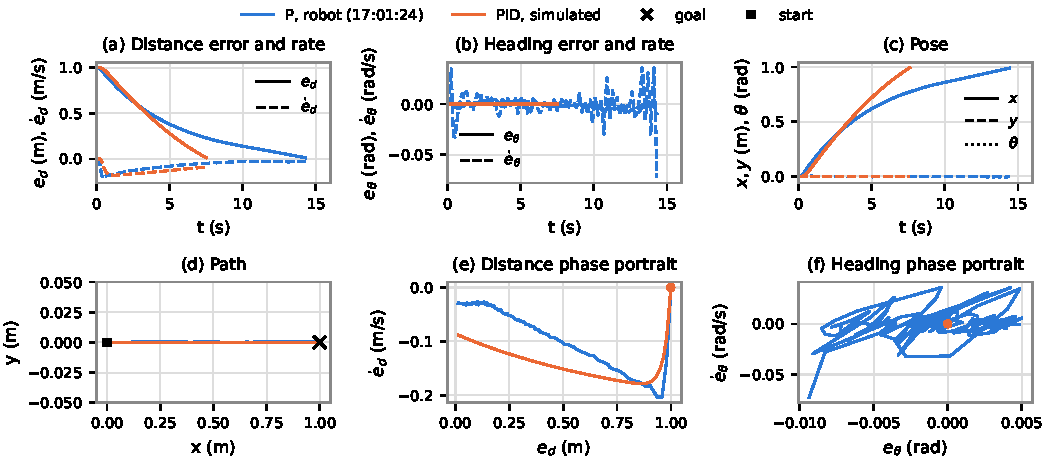
\includegraphics[width=\textwidth]{figures/fig_point_P.pdf}
  \caption{Point controller, goal 1\,m straight ahead, $k_{lp}=0.2$ (heading error below 0.6$^\circ$, so the heading gains play no
  part). Blue: P on the robot (17:01:24). Orange: our PID, same controller code, \textbf{simulated, not measured}, on a robot model
  fitted to run 17:12:26 (\texttt{sim\_point.py}). (a, b) $e$ and $\dot e$ vs time, (c) $x$, $y$, $\theta$ vs time, (d) path, (e, f)
  $\dot e$ vs $e$. Neither command reaches the 0.22\,m/s limit (PID peaks at 0.207\,m/s). P slows in proportion to $\ed$ and stops
  9\,mm short of the goal at 0.03\,m/s after 14.4\,s; the integral keeps PID faster: within 1\,cm after 7.6\,s, still at 0.09\,m/s.
  After the stop command the model rolls on for its delay and lag, after the logs end: PID ends $\approx$3\,cm past the goal, P
  $\approx$0.5\,cm. With a goal behind the robot the distance integral winds up during the turn and the simulated PID circles the
  goal, so we avoided it.}
  \label{fig:point}
\end{figure}

\para{Tuning process (Fig.~\ref{fig:tuning}).} \textit{(a) Distance gain.} When driving 1\,m straight ahead with unsaturated gains,
$\ed$ decays exponentially as predicted by a theoretical first-order model: fitted time constants 9.8\,s at $k_{lp}=0.1$ and 5.0\,s at 0.2
($1/k_{lp}$ = 10 and 5\,s). The last part of the graph turns into a straight line because the robot does not drive slower than about 0.03\,m/s
(lower end saturation is hit). To find where upper saturation starts we raised $k_{lp}$: from 0.3 the
command starts at the limit and quickly drops, and from 2.5 it stays there until the last 9\,cm (4.8\,s to the goal whatever the gain). We chose
$k_{lp}=0.2$, the largest gain that keeps $v=k_{lp}\ed$ below 0.22\,m/s for our 1\,m goals. \textit{(b) Heading gain, goal
behind the robot.} For a 180$^\circ$ turn, $\omega=k_{ap}\eh$ stays below 1.9\,rad/s only for $k_{ap}<0.6$. With 0.4 and 0.5 the
heading decays without overshoot (fitted time constants 4.1 and 2.6\,s vs $1/k_{ap}$ = 2.5 and 2\,s; slower than the ideal loop
because the bearing to the goal keeps moving while the robot drives sideways). This is because a lower $k_{ap}$ drives a wider arc (627 and 491\,mm), since the
distance loop drives forward during the turn. A saturated run ($k_{ap}=2.5$) turns faster (1.15\,s rise, 196\,mm arc) but overshoots
and hides the linear dynamics. We chose $k_{ap}=0.5$ for point goals behind the robot (run 17:12:26).

\begin{figure}[h]
  \centering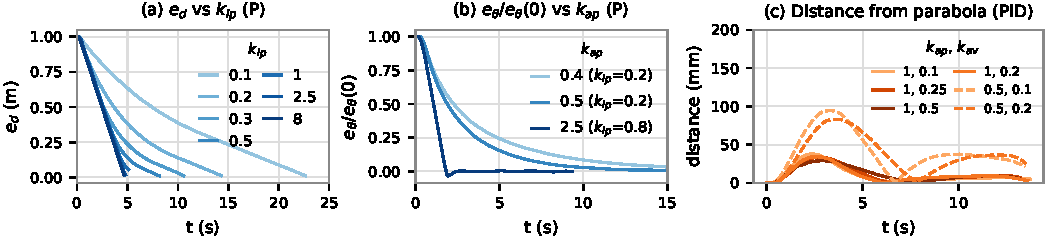
\includegraphics[width=\textwidth]{figures/fig_tuning.pdf}
  \caption{Tuning on the robot. (a) $\ed$ for seven values of $k_{lp}$ (P, goal 1\,m ahead). (b) Normalised heading error
  for three values of $k_{ap}$ (P, goal behind; the 2.5 run used $k_{lp}=0.8$, the others 0.2).}
  \label{fig:tuning}
\end{figure}

\para{Trajectories and choice of controller (Fig.~\ref{fig:traj}).} Most of our trajectory tuning went into the parabola (16 runs).
Because $\ed$ is measured to the end of the curve, P slows down over the last $v_{\max}/k_{lp}=1.1$\,m. With the same $k_{lp}$ and
$k_{ap}$, P, PI and our PID tracked the parabola similarly well (RMS 13--15\,mm, worst error in the tight first 0.5\,m), but the
integral term cut the time to come within 5\,cm of the end from 21.3\,s to 13.3--13.6\,s: it holds the speed command at the
0.22\,m/s limit for the whole run, so the robot does not slow down near the end. The D term gave the lowest worst-case deviation of
the three (34\,mm vs 37\,mm for PI and 40\,mm for P), so we chose PID for both trajectories. With a 1\,cm tolerance a PI run (17:53:25)
circled the end of the parabola: the integral keeps $v=0.22$\,m/s, and the tightest turn at that speed, $v_{\max}/\omega_{\max}=0.12$\,m,
cannot hit a 1\,cm circle, so the trajectory tolerance was set to 5\,cm. We stretched the sigmoid to $y=2/(1+e^{-x})-1$, $x\in[0,4]$
(lab: $2/(1+e^{-2x})-1$, $x\in[0,2.5]$), so that it leaves the origin at 27$^\circ$ instead of 45$^\circ$: the robot starts facing $+x$
and drives forward while it turns. Its worst error (59\,mm) is still at the start ($x=0.3$\,m); the RMS error is 20\,mm.

\begin{figure}[h]
  \centering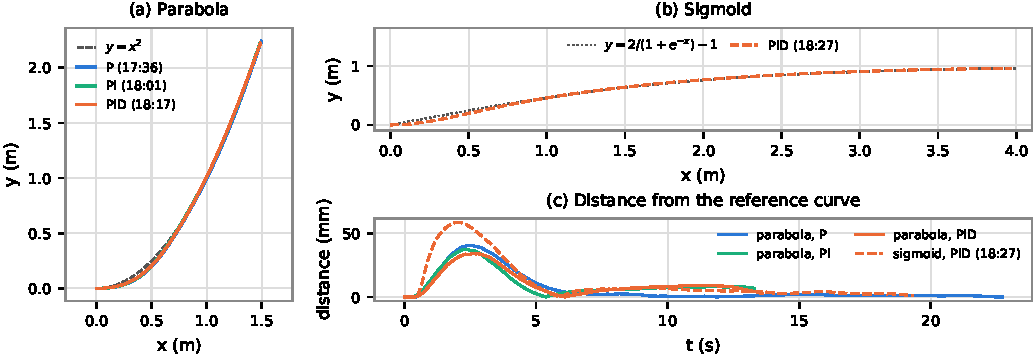
\includegraphics[width=\textwidth]{figures/fig_trajectories.pdf}
  \caption{Trajectories on the robot. (a) Parabola $y=x^2$, $x\in[0,1.5]$, with P (17:36:05), PI (18:01:56) and our PID (18:17:44) at the same $k_{lp}=0.2$, $k_{ap}=1.0$. (b) Sigmoid, stretched to $y=2/(1+e^{-x})-1$, $x\in[0,4]$, with our PID (18:27:45). (c) Distance from the robot to the reference curve. The P run used a 1\,cm end tolerance (PI, PID: 5\,cm); it was within 5\,cm of the end after 21.3\,s.}
  \label{fig:traj}
\end{figure}

%=====================================================================================================
\section{P vs PID point controller: stability analysis and discussion}

\begin{table}[h]
\centering\small
\caption{Point controller, goal 1\,m straight ahead, $k_{lp}=0.2$. P: measured on the robot (run 17:01:24). \textbf{PID: our PID,
simulated, not measured} (PID point runs were skipped on the TAs' recommendation due to limited lab time): the same controller code on
a robot model fitted to run 17:12:26. Rise time: distance from 90\,\% to 10\,\% of its start value. Settling: last exit from
$\pm5\,\%$. Times from the first command. Percent overshoot: peak past the goal of the linear model of the distance loop
(\texttt{expected\_pid.py}, below), which keeps controlling past the goal. The logs end inside the 1\,cm tolerance; the final position
adds the model's roll after the stop command (delay + lag). The heading error stays below 0.6$^\circ$, so only the distance loop is
compared.}
\label{tab:pvspid}
\begin{tabular}{llcc}
\toprule
 & Metric & P, measured & PID, simulated \\
\midrule
\multirow{3}{*}{Agility} & Rise time (s) & 10.6 & 5.6 \\
 & Settling time, 5\,\% (s) & 13.1 & 7.2 \\
 & Time to goal (s) & 14.4 & 7.6 \\
\midrule
\multirow{2}{*}{Accuracy} & Distance to goal at the stop command (mm) & 9.3 & 5.6 \\
 & Steady-state error & 0 & 0 \\
\midrule
\multirow{3}{*}{Overshoot} & Percent overshoot, linear model (\%) & 0 & 25 \\
 & Final position past the goal, est. (\% of 1\,m) & 0.5 & 3.3 \\
 & Speed at the goal (m/s) & 0.03 & 0.09 \\
\bottomrule
\end{tabular}
\end{table}

\para{Stability analysis.}
\textit{Distance loop.} With the heading aligned, $\dot\ed=-v$, so the robot itself is an integrator. P control gives $\dot\ed=-k_{lp}\ed$:
first order, time constant $1/k_{lp}$, no overshoot and zero steady-state error to a fixed goal. Our runs closely match: fitted time
constants 9.8, 5.0 and 3.2\,s for $k_{lp}$ = 0.1, 0.2 and 0.3 (theoretical 10, 5 and 3.3\,s; the 0.3 run is at the speed limit only for
its first 1.5\,s).
\textit{Heading loop.} The robot starts moving 0.2--0.6\,s after the first command (median 0.3\,s); modelling this as a lag
$\tau\approx0.2$\,s gives $\tau\ddot\eh+(1+k_{av})\dot\eh+k_{ap}\eh=0$ and $\zeta=(1+k_{av})/(2\sqrt{k_{ap}\tau})$. Our P gains
$k_{ap}=0.4$--0.5 give $\zeta=1.8$--1.6: overdamped, and we measured no overshoot. As a check on $\tau$, the saturated $k_{ap}=2.5$ run
($\zeta=0.71$, predicted 4.3\,\%) overshot by 3.4\,\%.
\textit{Our PID.} With the I term the distance loop becomes $(1+k_{lv})s^2+k_{lp}s+k_{li}=0$: $\zeta=0.62$ for our $k_{li}=0.025$, so the
overdamped P loop becomes slightly oscillatory ($\zeta\geq0.7$ would need $k_{li}\leq0.019$). In this linear model $\ed$ reaches zero
after 7.3\,s at 0.08\,m/s and then overshoots by 25\,\%; the simulation in Table~\ref{tab:pvspid} agrees on the arrival (7.6\,s,
0.09\,m/s), and stopping at the 1\,cm tolerance cuts the overshoot to the roll after the stop command. In the heading loop
($k_{ap}=1.0$) P alone gives $\zeta=1.12$; the D term raises it to 1.34, and the I term adds a slow mode (time constant 39\,s) and a
2.6\,\% overshoot on a 180$^\circ$ turn. The two loops are coupled, though: with a goal behind the robot the distance integral winds up
during the turn, and the simulated PID circles the goal at full speed instead of stopping.

\para{Discussion.}
\textit{Agility:} the I term makes the distance loop about twice as fast (rise 5.6 vs 10.6\,s, goal after 7.6 vs 14.4\,s): as $\ed$
shrinks, the integral keeps the speed up where P slows down in proportion to $\ed$. On the parabola the same effect cut the time from
21.3 to 13.6\,s.
\textit{Accuracy:} the robot integrates the speed command, so P already has zero steady-state error to a fixed goal; both controllers
stop inside the 1\,cm tolerance, and the I term adds no accuracy.
\textit{Overshoot:} PID arrives at 0.09\,m/s instead of 0.03\,m/s, so it ends $\approx$3\,cm past the goal instead of $\approx$0.5\,cm,
and the linear model predicts a 25\,\% overshoot if it did not stop. It also fails for a goal behind the robot.

For a fixed goal we would therefore use P, or PID only with an integral clamp and the goal ahead of the robot; we would add D only if a
higher $k_{ap}$ made the heading underdamped (above $k_{ap}\approx1.25$ for $\tau=0.2$\,s). For trajectories PID is the better choice:
the speed the integral adds shortens the run without hurting tracking, and the 5\,cm end tolerance absorbs the arrival speed. The wide
arc at the start of the sigmoid comes from driving while turning; scaling the speed by $\cos\eh$ would remove it. P with $k_{ap}=3.0$
tracked the parabola tightest (8\,mm, 23.1\,s), so a higher $k_{ap}$ is the next PID tuning step.

\end{document}
